\section{What's the Matter}

\begin{quotex}
\emph{Law 1}. A body continues in its state of rest, or in uniform motion in a straight line, unless acted upon by a force. \flright{\textsc{Isaac Newton}}

The correlative of Purusha is then Prakriti, the undifferentiated primordial substance; it is the passive principle, which is represented as feminine, while Purusha is the active principle, represented as masculine; and these two are the poles of all manifestation, though remaining unmanifested themselves. \flright{\textsc{Rene Guenon}, \emph{Man and his becoming}}

\end{quotex}
Newton's first law shows that \textbf{matter} cannot cause an event; on the contrary, it is entirely passive. Only and external force can change its motion, or set it in motion. Although subsequent developments (e.g., Euler, Relativity) have generalized Newton's law, the fundamental point remains: matter is passive. Hence, matter cannot create anything in an active sense. What about the force that alters matter? This is energy as defined:

\begin{quotex}
\textbf{energy} is the quantitative property that must be transferred to a body or physical system to perform work on the body. \flright{\textsc{Wikipedia}}

\end{quotex}
That is not a particularly helpful definition. All it says is that energy is the ability to do work, that is, to change the motion of a material object. It does not say what energy ``is" but only what it does. We infer it either through the motions of matter or the experience of heat.

It is known that matter and energy are convertible. At the moment of creation, there was only energy. As the energy, in the form of photons, spread out, the universe cooled When it cooled sufficiently, energy converted to matter. Hence, matter is condensed energy.

\paragraph{Will}
Everything that we know about the world necessarily begins with our sense experience of it.  We touch, see, hear, smell, and taste things. We notice that things move, develop, change direction. One of these things is our own body. We can experience our body as a thing in the world.

But we can experience our own body in a unique way, in a way that we cannot experience any other thing. That is in its interiority. I experience my Will independent of any sensory experience of my body. I can see that the Will gathers up and focuses energy in order to cause my body to move. Hence, at the most fundamental level, we have this schema:

\begin{enumerate}
\item Will 
\item Energy is condensed Will 
\item Matter is condensed Energy 
\end{enumerate}
\paragraph{Subatomic Particles}

\begin{wrapfigure}{rt}{.3\textwidth}
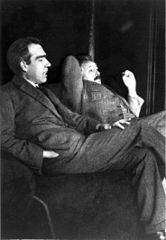
\includegraphics[scale=.5]{a20211212WhatstheMatter-img001.jpg}
\caption{Niels Bohr and Albert Einstein disputing the nature of reality.}
\end{wrapfigure}

That is a different conception of matter, yet not incompatible with physics as understood. Before quantum theory, matter was defined as that which has extension, i.e., volume. It takes up space. Taking up space is an illusory epiphenomenon of the properties of some subatomic particles like fermions. Thus, in the Standard Model of Physics, the quantum entities do not have size, volume or extension.

Mass, then, is the fundamental property of matter. Mass has a well-defined scientific definition, but matter does not; it is a vague term.

Fermions have properties such as mass, charge, spin, and a few others. No two particles can occupy the same state. A subatomic particle does not exist at a particular place. Rather the possible states of a particle are described via a probability distribution. Thus, an electron can be at any of the places, some obviously more likely than others. That means an electron may be a million miles away, although that is quite unlikely even if mathematically possible. Moreover, there are gaps in which the electron cannot exist at all.

\paragraph{Measurement Problem}
From the above discussion, fundamental matter is nothing in particular. Matter is just a collection of particles in given states and probability distributions. So what happens when you ``look" at matter? Suddenly, one of the possible states of matter becomes actual. This is called the ``measurement problem" in quantum mechanics. Physicists do not have a firm grasp of what exactly is happening with the ``quantum measurement problem", so we'll leave it up to them to resolve. The point is that matter is not so simple to understand.



\flrightit{Posted on 2021-12-12 by Cologero }

\begin{center}* * *\end{center}

\begin{footnotesize}\begin{sffamily}



\texttt{veritycacciatrice on 2021-12-15 at 06:20 said: }

Reminds me of something I read once.

If one imagines an empty soda can grasped at both ends and twisted in opposite directions it creates a crumpling effect on the can. (Torsion.)

When the unperturbed ether or lattice structure of empty (or waiting, or Nyx's empty womb-like) space has consciousness hit it from a couple of directions, the lattice structure is crumpled slightly at the point where the interference pattern meets like two stones dropped in a pond whose ripples join up from a few meters away. The stronger the consciousness, the greater the torsion, until matter forms.

It might be as simple as two consciousnesses from a distance thinking of each other, say workers in an office, who then become obsessed with each other, get married and have a baby.

They created their baby from where there was `nothing' before, but/and consciousness was the first step.


\hfill

\texttt{Max on 2021-12-19 at 15:32 said: }

Newton sat under a tree. A serpent dropped an apple on his head. Its impact caused Newton to think: ``the apple fell in a straight line, it would have continued to fall forever unless my forceful head stopped it". Then he got angry: ``I was in a state of rest, wich I could have continued forever, if not for the straight fall of the apple." Much disturbed, he reluctantly got up, and penned down that nothing ever happens unless a force forces it to happen. Then he took a big bite, ``You force me to do this, serpent, you are the cause why things fall." As it slithered away, a quiet whisper that ``It all depends on the frame of reference," could be made out.

``Newton, blind fool, your laws are like the particles of dust you crawl in." The law is an invention, not an observation, and it does not show anything other than your own image. Matter altering energy, energy altering matter. If they are convertible, and matter cannot cause an event, then energy cannot cause an event either. A difference of degree but not kind. Then there must be a non-force acting on force and mass. It seems that a body continues to deteriorate and be restless, never going in a straight line, unless acted upon by a non-force.

A particle – sub-indivisible or not – that cannot be at a specific place, logically cannot be at one of a number of different ``probable" places either. The first negation invalidates the entire probability distribution. It will consequently never fall in a straight line on innocent heads, regardless of how many times it is tried. Only by false belief and illusion does the serpent sprinkle distracting particles before the guilty. The probability of the particle being at any of the places is zero. Particulars exist, but ``particles" is a reification. Matter is not a particular or a collecton of reified particles.

Perhaps physicists with their measurement problems came across the immeasurable, but did not understand immeasurability. At any rate, no amount of measuring will make the immeasurable measurable. As a hypothetical scenario, we try to measure something that does not exist, and get a positive reading on our instrument. The first order is to determine whether we are now faced with an existential problem, a measurement problem, or an intellectual problem.


\end{sffamily}\end{footnotesize}
